\chapter{Deep Learning}
\label{cha:dnn}
Deep Learning research in the field of artificial neural networks~(ANNs) has dominated state-of-the-art solutions on cognitive tasks, e.g. the performance exceeding human-level  on image classification tasks~\citep{he2015delving} and playing GO~\citep{silver2016mastering}).
Merging deep learning techniques into SNNs may provide an answer to the problem of how to operate SNNs to perform as well as ANNs in cognitive tasks. 
In this chapter, we will give an overview of popular architectures and models of deep learning in Section~\ref{sec:dl_history}, and the rest of this chapter will illustrate the mechanisms of convolutional networks (ConvNets), autoencoders (AEs), and restricted Boltzmann machines~(RBMs) in detail which will be used in following chapters.

\section{Brief Overview}
\label{sec:dl_history}
Deep learning seems to have become the answer to all artificial intelligence problems overnight since Geoffrey Hinton proposed the training method of a type of ANN, deep belief network, in 2006~\citep{hinton2006fast}.
However, deep learning is not a new `magic', but rather has a history over a few decades and its sudden success is the result of the availability of an increasing amount of training data, growing size of network models and greater computational power.
Therefore, all the classical deep learning architectures date back to the last century when deep learning un-named.
However, at that time, deep networks were hardly to be trained mainly because of the limit on computational power.


\subsection{Classical Models}
We call the well-known and widely-used deep learning models `classical' and give a brief introduction to those models in this section. 
As mentioned above, the first break-through of training deep, not shallow ($\le 3$ layers), networks was the greedy layer-wise strategy~\citep{hinton2006fast} proposed to train stacked RBMs, which will be described in more detail in Section~\ref{sec:rbm}.
Shortly after that this method was proved to be efficient for training other kinds of deep networks including stacked AEs~\citep{bengio2007greedy} (stated in Section~\ref{sec:AE}).
RBMs and AEs are suitable for dimensionality reduction and feature extraction when trained with unsupervised learning on unlabelled data.
In 2012, using such a unsupervised deep learning architecture the Google Brain team achieved a milestone in the deep learning era; the neural network learned to recognise cats by `watching' 10 million images generated from random frames of YouTube videos~\citep{le2013building}.

ConvNets are biologically inspired from the significant discovery of Hubel and Wiesel that the orientation selectivity (simple cells) and pooling mechanism (complex cells) represent the basic functions in the primary visual cortex in cats~\citep{hubel1962receptive}.
These simple cells fire at a high frequency to their preferred orientation of visual stimuli within their receptive fields~(shown in Figure~\ref{Fig:v1}), small sub-regions of the visual field.
%This means a single simple cell works like a pattern detector within its small receptive field thus also providing the exact spatial location of the detected feature in the entire visual field.
Meanwhile, a complex cell corresponds to the existence of a pattern within a larger receptive field but loses the exact position of the pattern.
%This means that its receptive field cannot be mapped into fixed excitatory and inhibitory zones. Rather, it will respond to patterns of light in a certain orientation within a large receptive field, regardless of the exact location.
%The receptive fields composes of the entire visual field.
%These cells act as local filters over the input space and are well-suited to exploit the strong spatially local correlation present in natural images.
NeoCognitron~\citep{fukushima1982neocognitron} was the first to mimic the functions of V1 simple and complex neurons in an artificial neural network, and later this feature detection of single cells was improved by sharing weights among receptive fields in LeNet-5~\citep{lecun1998gradient}, the typical ConvNet used today.
The mechanism of shared weights forms the essence of convolution in a ConvNet, which hugely reduces the number of weight parameters in a network.
The most significant milestones produced by deep ConvNet dominated the best performances in the annual ImageNet Challenge~\citep{russakovsky2015imagenet}: AlexNet~\citep{krizhevsky2012imagenet}, VGG Net~\citep{simonyan2014very}, GoogLeNet~\citep{szegedy2015going} and ResNet~\citep{he2016deep}.

Despite the powerful capabilities of these feed-forward deep networks, sequence processing is a challenge for them since the input and output vectors are of static size.
Thus recurrent neural networks~(RNNs), containing feed-back connections, are ideal solutions for dealing with sequential information since their current output is always dependant on the previous `memory'.
As training mechanisms have become more mature, for example using the long short-term memory or (LSTM)~\citep{hochreiter1997long}, RNNs have shown great success in many natural language processing tasks: language modelling~\citep{mikolov2010recurrent}, machine translation~\citep{sutskever2014sequence}, speech recognition~\citep{graves2014towards} and image caption generation~\citep{karpathy2015deep}.

\subsection{Combined Approaches}
Current trend of deep learning is to combine machine learning algorithms towards more complex objectives: such as decision making and data generation.

Reinforcement learning (RL) is inspired from animal behaviour when agents learn to make sequential optimised decisions to control an environment.
To address complex decision making problems in practical life, RL requires a sufficiently abstract representation of the high-dimensional environment, where deep learning is exactly clever at dimensionality reduction and feature extraction.
The milestone achieved by integration of RL and deep networks, the deep reinforcement learning, drew everyone's attention on artificial intelligence when AlphaGo beat a professional human player in Go~\citep{silver2016mastering}.
%which has been successfully applied to various tasks: such as games~\citep{mnih2015human}, robotics~\citep{schulman2015trust} and question-and-answer systems.
%Potential in real-time neuromorphic system
%These real-time decision making systems, especially used for robotics~\citep{schulman2015trust}, are ideal for meromorphic hardware systems which takes advantages in event-based processing and energy efficiency.
%http://blog.aylien.com/introduction-generative-adversarial-networks-code-tensorflow/

Generative Adversarial Networks (GANs)~~\citep{goodfellow2014generative} are proposed for training generative models of complex data.
Instead of training discrimination networks (e.g. image classification using CovNets ) and generation networks (e.g. data sampling on RBMs) separately with different objectives, GANs train two competing networks, one the discriminator, the other the generator, simultaneously by continuously using them to play games with each other.
Thus, the generator learns to produce more realistic data to cheat the discriminator; meanwhile the discriminator learns to become better at distinguishing generated from real data.
Exciting achievements have been reported on generating complex data such as realistic image generation based on description in text~\citep{radford2015unsupervised}.

\section{Convolutional Networks}
\label{sec:convnet}
In Chapter~\ref{cha:Conv}, we will use a convolutional network to demonstrate a training method on spiking deep architectures.
This section aims to give a detailed introduction to ConvNet architectures and its training with back propagation.
\subsection{Network Architecture}

	\begin{figure}[bt]
		\centering
		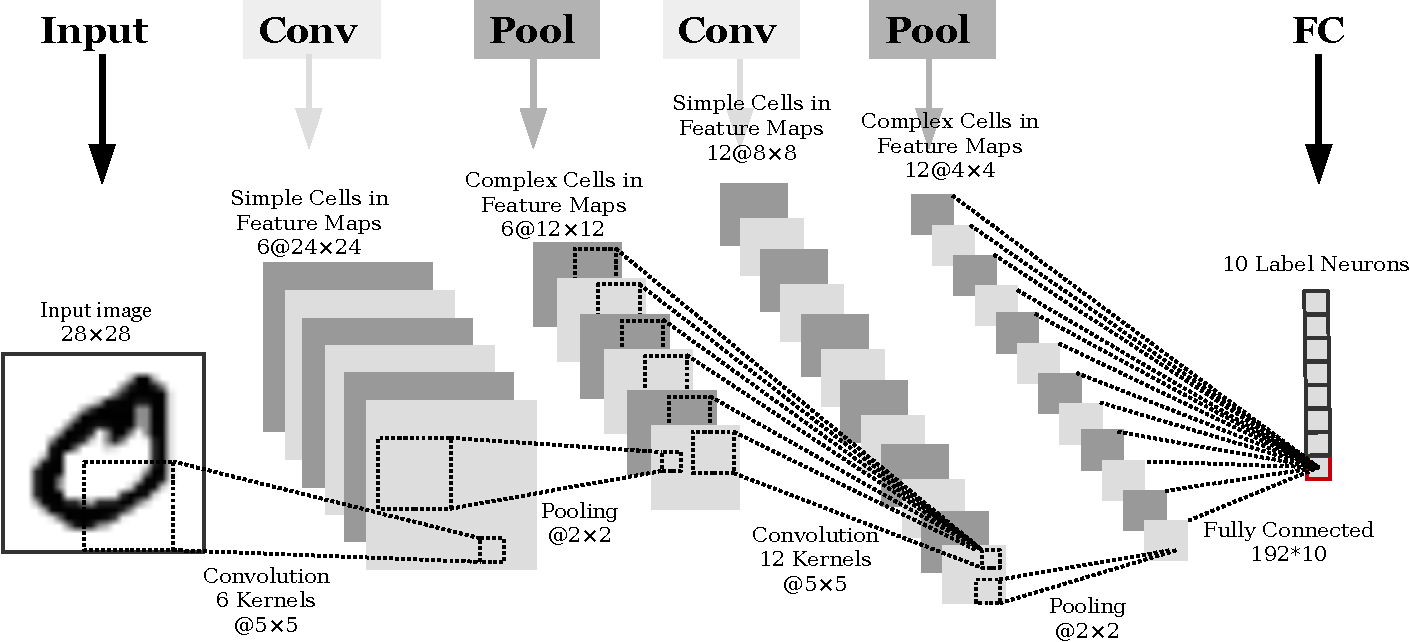
\includegraphics[width=0.95\textwidth]{pics_snn/convnet.pdf}
		\caption{Typical ConvNet architecture.}
		\label{Fig:ConvNet}
	\end{figure}

A typical ConvNet (LeNet) consists of four types of neural layers: an input layer, convolutional~(Conv) layers of simple cells, pooling layers of complex cells and fully-connected~(FC) layers, as shown in Figure~\ref{Fig:ConvNet}.
From the left to right of Figure~\ref{Fig:ConvNet}, we illustrate the mechanism of ConvNet in detail.

The pixels of the input image are normalised and fed into the first Conv layer.
Every simple cell takes inputs within its receptive field and the weights on each input pixel are determined by the convolutional kernel which has the same size as the receptive field.
The neurons work as demonstrated in Figure~\ref{Fig:compare_as}(a) performing a dot product between the weights and the input volume of a receptive field; this is followed by an activation function.
Convolving a whole input image with a kernel composes a feature map in the Conv layer, thus there are 6 feature maps in the first Conv layer.
Stride controls the output volume of a convolution such that setting the stride to $step$ causes the kernel moving $step$ pixels at a time.
Thus a small stride produces more output volume and highly overlapping receptive fields.
Suppose an input image and a kernel are both squares with side lengths of $l_{in}$ and $l_k$, then the side length of the convolved feature map is $(l_{in} - l_k + 1)/stride$.

The special characteristics of Conv layers lie in the local connectivity and the parameter sharing, such that a neuron connects only to a spatially local input volume, its receptive field; and the weights (convolutional kernel) are shared among all the receptive fields.
Consequently, the number of parameters (trainable weights) hugely decreases compared to all-to-all connections of same network size. 

The complex neurons of pooling layers either output the maximum input within their receptive fields (max pooling) or the averaging (average pooling), as applying a max/average filter to non-overlapping receptive fields.
The pooling process reduces the spatial size of the feature maps but keeps the number of features.
In Chapter~\ref{cha:Conv}, we will use average pooling of $2\times2$ for all the pooling layers, shown in Figure~\ref{Fig:ConvNet}.
The average filter traverses over an entire feature map with a stride of 2, and outputs the averaged element of each receptive field to the next layer.

The next Conv layer drives 3D feature vectors with a depth of 6 (six feature maps) to convolve with 12 3D kernels with size of $6\times5\times5$.
The example demonstrates a common set-up using the whole 3D feature vectors; usually the feature maps can be selected to be involved in different convolutions.
Then a pooling layer follows the convolution.
Repeating these alternative presentation of a Conv layer and a pooling layer builds up deeper ConvNet.

The trainable shared weights used in the Conv layer hugely reduces the number of weight parameters in a ConvNet, while pooling layers use static convolutional kernels to shrink the size of networks.
These convolutional connections can be described as 6c5-2s-12c5-2s, where $\alpha c \beta$ indicates $\alpha$ kernels of side length $\beta$ used in Conv layer, and $2s$ specifies the side length and the stride of a pooling kernel.
However, a multilayer perceptron (MLP) network possesses only FC layers, where each neural layer fully connects to the next one.
In a ConvNet an FC layer is usually located on the top (right in Figure~\ref{Fig:ConvNet}) of a network, connects the last pooling layer to the output neurons with all-to-all connections and predicts the classification of the input image.
The strongest output among the label neurons addresses to which class the input image belongs, as illustrated in Figure~\ref{Fig:ConvNet} where the red neuron represents the first digit out of ten, `0'.
There can be more than one FC layers consisting a MLP on the top of a ConvNet, in this thesis, we will use only a single FC layer.


%Chain rule, reduced parameter amounts. 

\subsection{Backpropagation}
We have described the feed-forward path of a ConvNet to classify an input image, this section will demonstrate the training of a network by back-propagating errors and weights modification.
The objective function (or loss function) estimates an error comparing the output vector of a network, $\mathbf{y}=(y_1,y_2,...,y_M)$, to the desired label vector, $\mathbf{t}=(t_1,t_2,...,t_M)$, and the error is to be minimised during training.
Given a set of training data with desired labels $\mathbf{T}=\{\mathbf{t}^1, \mathbf{t}^2, ..., \mathbf{t}^K\}$ and the network output $\mathbf{Y}=\{\mathbf{y}^1, \mathbf{y}^2, ..., \mathbf{y}^K\}$ the mean squared error can be seen as the objective function:  
\begin{equation}
L=MSE(\mathbf{T}, \mathbf{Y}) =\frac{1}{2K}\sum_{k=1}^K \sum_{m=1}^M (y^{k}_{m}-t^{k}_{m})^{2}~~.
\label{equ:loss_all}
\end{equation}

Backpropagation~(BP), propagates the gradient of the loss with respect to the weights backwards to each connection in the network.
The computation requires a closer look into the structure of a neuron, see Figure~\ref{Fig:neuron_net} where $N$ neurons connect to the $j^{th}$ neuron of the next layer, and the neuron converts the weighted summation of the input, $net_j$, to the output $y_j$ according to its activation function.
\begin{figure}[bt]
	\centering
	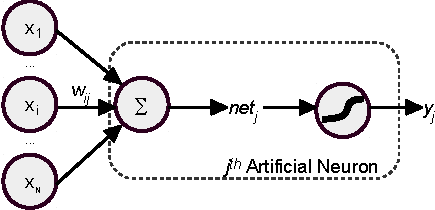
\includegraphics[width=0.7\textwidth]{pics_iconip/neuron.pdf}
	\caption{ $N$ neurons connect to the $j_{th}$ neuron of the next layer. As illustrated in Figure~\ref{Fig:compare_as}(a), we use simplified artificial neuron without bias.}
	\label{Fig:neuron_net}
\end{figure}
Thus the gradient of the loss $L$ with respect to a weight $w_{ij}$ is as follows:
\begin{equation}
\begin{aligned}
\frac{\partial L}{\partial w_{ij}} &= \frac{\partial L}{\partial y_j} \frac{\partial y_j}{\partial net_j} \frac{\partial net_j}{\partial w_{ij}} = \delta_j x_i , \textrm{~~where~~}\\
 \delta_j &=  \frac{\partial L}{\partial y_j} \frac{\partial y_j}{\partial net_j}~~,  \textrm{~~and~~}\\
% \frac{\partial y_j}{\partial net_j} &= f'(net_j)~~, \\
 \frac{\partial net_j}{\partial w_{ij}} &= x_i~~.
\end{aligned}
\end{equation}
The term $ \delta_j $ represents the error gradient with respect to $net_j$, and can be expressed by a recursive definition:
\begin{equation}
\begin{aligned}
\delta_j =  \frac{\partial L}{\partial y_j} \frac{\partial y_j}{\partial net_j} &= \left\{
\begin{aligned}
&\frac{1}{K}\sum_{k=1}^K (y^{k}_{j}-t^{k}_{j}) f'(net_j)  \textrm{~,~~if \textit{j} is in an output layer} \\
&(\sum_l^L \delta_l w_{jl}) f'(net_j)  \textrm{~,~~if otherwise}
\end{aligned}
\right. \textrm{~,~~where}\\
 \frac{\partial y_j}{\partial net_j} &=  f'(net_j) \textrm{~,~~the derivative of the activation function}.
\end{aligned}
\label{equ:derivative}
\end{equation}
It is easy to obtain the first term, $ \frac{\partial L}{\partial y_j}  $, of $ \delta_j $ if $j$ is an output neuron since it only involves single dimension of the output vector.
However, when $j$ is in an inner layer of the network, which connects $L$ neurons on the next layer, we have to take total derivative with respect to $y_j$: $\sum_l^L \delta_l w_{jl}$.
The error propagation applies to any form of connection in a network, such as FC and Conv layers, and the difference only appears in the summation where matrix product is used for the FC layer and convolution for Conv layer.
In addition, the weights used in BP are either transposed in FC layer or rotated in Conv layer compared to the forward path.

After error propagation, the BP algorithm updates weights using the optimisation method, gradient descent, to minimize the objective function.
It modifies the weights by small steps proportional to the negative of the gradients:
\begin{equation}
\Delta w_{ij} \propto -\frac{\partial L}{\partial w_{ij}} = -\eta \delta_j x_i~~,
\label{equ:delta_w}
\end{equation}
where $\eta$ defines the length of these updating steps which is also called learning rate.
Again, the weight update is also dependant on the types of layers, where a convolution of the input vector $\mathbf{x}$ with the error gradient  $\mathbf{\delta}$ is needed in Conv layers.
A detailed description of BP training on ConvNet can be found in~\citep{bouvrie2006notes}.

Moreover, applying stochastic gradient descent (SGD), the gradient over the full training set can be approximated using only a single or a few training data.
Therefore $k$ in Equation~\ref{equ:derivative} can be seen as a randomly selected data index, and $K$ represents the number of elements in such a data subset, which is also known as a batch.
If we take only one data sample in each batch, the loss function~(Equation~\ref{equ:loss_all}) will be estimated by the error between an output vector $\mathbf{y}^k$ and the single label sample $\mathbf{t}^k$:
\begin{equation}
E^k = \frac{1}{2}\sum_{m=1}^M (y^{k}_{m}-t^{k}_{m})^{2}~~,
\label{equ:error_conv}
\end{equation}
and the equation can be simplified by deleting the index $k$, assuming the error is computed for each data sample:
\begin{equation}
E = \frac{1}{2}\sum_{m=1}^M (y_{m}-t_{m})^{2}~~.
\label{equ:error_non}
\end{equation}


\subsection{Activation Function and Vanishing Gradient}

%\begin{figure}[hbt]
%	\centering
%	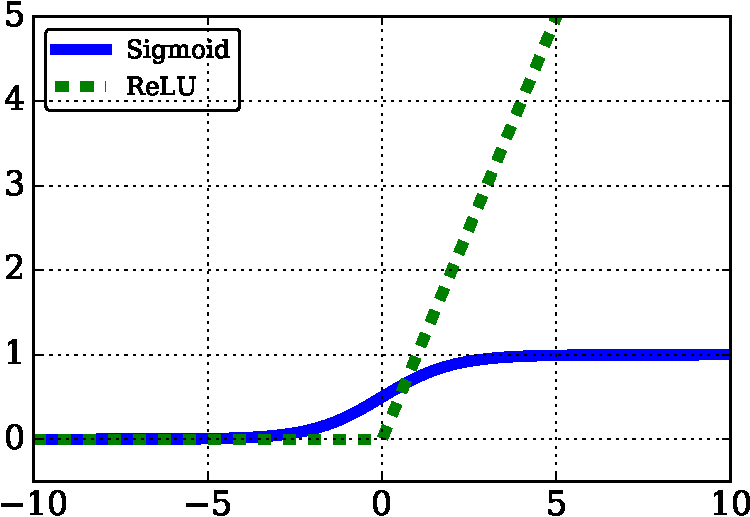
\includegraphics[width=0.6\textwidth]{pics_snn/af.pdf}
%	\caption{Activation functions: sigmoid and ReLU.}
%	\label{fig:af}
%\end{figure}

\begin{figure}[tbp!]
	\centering
	\begin{subfigure}[t]{0.48\textwidth}
		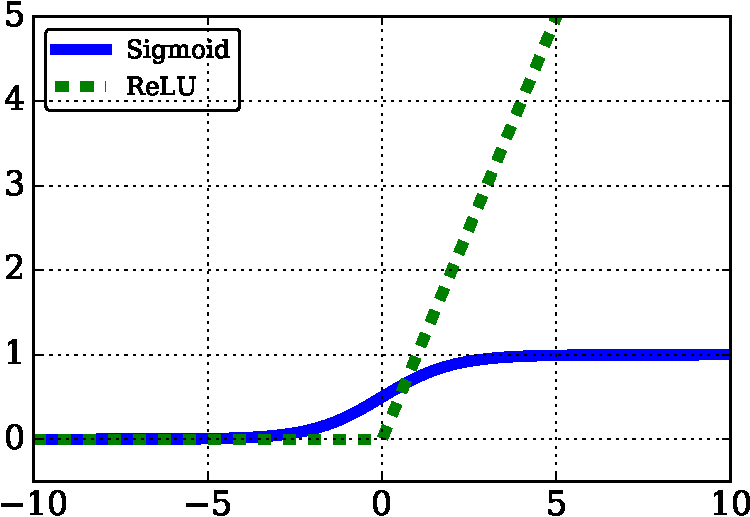
\includegraphics[width=\textwidth]{pics_snn/af.pdf}
		\caption{Activation functions}
	\end{subfigure}
	~~
	\begin{subfigure}[t]{0.48\textwidth}
		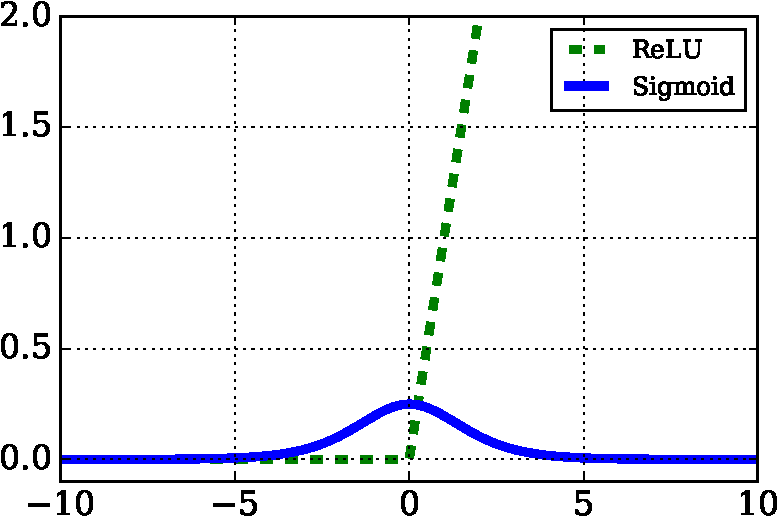
\includegraphics[width=\textwidth]{pics_snn/af_der.pdf}
		\caption{Derivatives of the activation functions}
	\end{subfigure}
	\caption{Activation functions: (a) sigmoid and ReLU, and (b) their derivatives.}
	\label{fig:af}
\end{figure}
Each error gradient propagated through layers of network consists of a chain of multiplied factors as illustrated in Equation~\ref{equ:derivative}.
The deeper a network is and the closer a layer is to the input, the more elements are involved in the multiplication including the derivative of the activation function.
%The derivative of the activation function is a recursive factor in the BP chain, 
%one of the factors when the error gradient back propagated in each layer.
Thus, the gradient may vanish if the derivative of the activation function is always less than 1.
For the sigmoid function example, shown in Figure~\ref{fig:af}(a), its derivative keeps the maximum (around~0.25) only when the input is close to 0, and decays to its minimum 0 as the input either increases or decreases, see Figure~\ref{fig:af}(b).

Rectified Linear Unit (ReLU) is proposed to tackle the problem of vanishing gradient in deep networks.
ReLU, simply defined as $y = max(0,x)$ and shown in Figure~\ref{fig:af}, has a gradient of 1 when the input is greater than 0.
Hence, the error gradient is able to be back-propagated in deeper network by multiplying ReLU derivatives.

\section{Autoencoders}
\label{sec:AE}
Autoencoders are categorised as unsupervised learning, since AE aims to reconstruct its original input as closely as possible.
Thus the output and input vectors have the same dimensionality.
But the hidden middle layer is allowed to have either more, or fewer, neurons for the purpose of compressing the inputs or mapping them to higher dimensions.
Hence AE is suitable to learn effective representation of the original inputs at the hidden layer, which can be seen as the encoding phase of AE, and reconstruct them on the output layer where the hidden vectors are decoded. 

Multiple AEs can be stacked to build deep AEs where the hidden layer of a lower AE represents the input of the upper block, and each AE block can be trained individually with greedy layer-wise training~\citep{hinton2006fast}.
A stacked AE takes advantage of greater expressive power as does any deep network.
Taking image processing as an example, the lower AE blocks learn only simple features, such as edges and dots, however on the upper layers more complicated and abstract features are extracted: contours, symbols and even objects. 

In this section, we will only describe the structure and training method of single AE blocks, since the greedy layer-wise training on stacked AEs is no different from training multiple single AEs except for different input data.
Due to AE's simple network architecture and training algorithm, spiking AEs will be built and trained with biologically-plausible training mechanism in Chapter~\ref{cha:sdlm}.

\subsection{Structure}
Figure~\ref{fig:AE} shows the architecture of an AE, which is an MLP consisting of three layers of neurons: visible ($\mathbf{v}$), hidden ($\mathbf{h}$) and reconstruction ($\mathbf{v'}$) layers.
Both visible and reconstruction layer have $N$ dimensions, and the hidden layer has $M$.
Note that AEs usually have tied weights where the connections ($\mathbf{w}^T$) between $\mathbf{v}$ and $\mathbf{h}$ are transposed to form the connections ($\mathbf{w}$) from $\mathbf{h}$ to $\mathbf{v'}$.


\begin{figure}
	\centering
	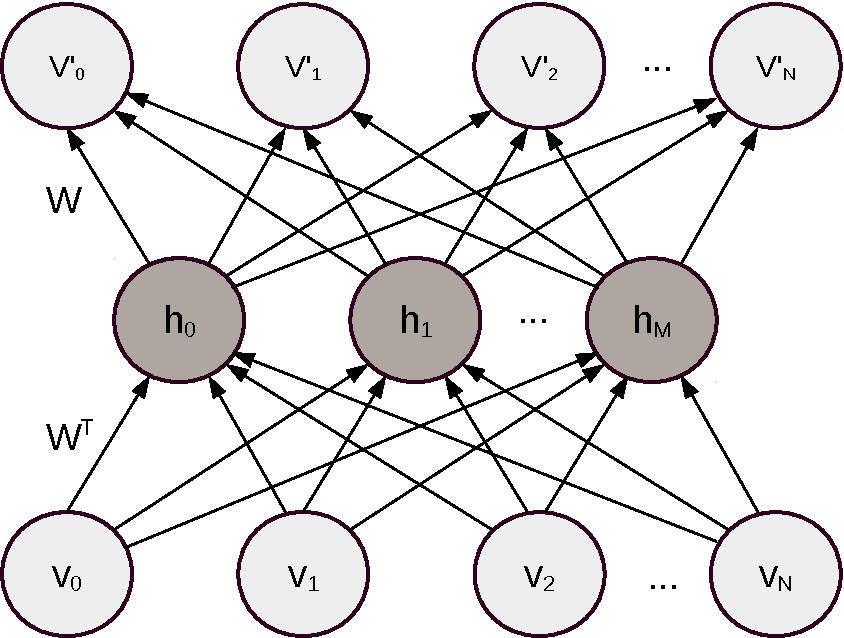
\includegraphics[width=0.5\textwidth]{pics_sdlm/AE.pdf}
	\caption{A typical Autoencoder structure.}
	\label{fig:AE}
\end{figure}


\subsection{Training}
The feedforward path of an AE, as for an MLP, non-linearly transforms the input through two FC layers, where each neuron performs weighted summation and activation as illustrated in Figure~\ref{Fig:neuron_net}.
Training an AE is also similar to that for an MLP, however, the difference lies in the objective where the AE aims to minimise the difference between the input $\mathbf{v}$ and its reconstruction $\mathbf{v'}$, instead of between the output and some labelled data (supervised learning).
Therefore the loss function generated by single data sample $\mathbf{v}$, described in Equation~\ref{equ:error_non} for supervised learning, is as follow:
\begin{equation}
E = \frac{1}{2}\sum_{n=1}^N (v'_{n}-v_{n})^{2}~~,
\end{equation}
and the weight update, shown in Equation~\ref{equ:delta_w}, is proportional to the error gradient with respect to the weight:
\begin{equation}
\Delta w_{ij} \propto -\frac{\partial E}{\partial w_{ij}} = -\eta \delta_j h_i~~,
\end{equation}
where $\eta$ is the learning rate, $h_i$ is the hidden neuron and the term $\delta^k_j$ is the error gradient with the respect to $net_j$, the weighted summation.
The weight tuning needs only to be applied in the reconstruction layer, since study~\citep{xu1993least} has proved that updating the transposed weights $\mathbf{w}^T$ at the hidden layer does not improve the learning and the error gradients are usually small.
Hence, $\delta^k_j$  can be calculated according to Equation~\ref{equ:derivative}:
\begin{equation}
\delta_j = (v'_{j}-v_{j}) f'(net_j)~~,
\end{equation}
and the weight update can be simply described by:
\begin{equation}
\Delta w_{ij} = \eta h_i (v_{j}-v'_{j})  f'(net_j)~~.
\end{equation}
If we use ReLU as the activation function, then the above equation is as follow:
\begin{equation}
\label{equ:ae_widrow_hoff}
\Delta w_{ij} = \left \{
\begin{aligned}
& \eta h_i(v_j - v'_j)~, & net_j > 0 \\
& 0~, & net_j < = 0
\end{aligned} 
\right.
\end{equation}

%\begin{equation}
%\begin{aligned}
%\Delta w_{ij} = -\eta \frac{\partial E_k}{\partial w_{ij}} &= -\eta \frac{\partial E_k}{\partial v'_j} \frac{\partial v'_j}{\partial net\_v'_j} \frac{\partial net\_v'_j}{\partial w_{ij}}, \textrm{ where} \\
%\frac{\partial E_k}{\partial v'_j} &= \frac{\partial \frac{1}{2} \sum_l (v_l - {v'}_l)^2}{\partial v'_j}= \frac{\partial \frac{1}{2}(v_j - {v'}_j)^2}{\partial v'_j}= v'_j - v_j, \\
%%	\frac{\partial v'_j}{\partial net\_v'_j} &= \begin{cases} 1, v'_j>0\\0, v'_j<=0\\ \end{cases}, \textrm{using ReLU,}\\
%%\frac{\partial v'_j}{\partial net\_v'_j} &=\left\{
%%\begin{aligned}
%%& 1, net\_v'_j > 0 \\
%%& 0, net\_v'_j < = 0
%%\end{aligned} 
%%\right.    \textrm{using ReLU, }\\
%\frac{\partial v'_j}{\partial net\_v'_j} &= f'(net\_{v'_j})~, \textrm{~derivative of the activation function} \\
%\frac{\partial net\_v'_j}{\partial w_{ij}} &= \frac{\partial h_i w_{ij}}{\partial w_{ij}} = h_i.
%\end{aligned}
%\end{equation}
%Thus, the weight gradient is calculated as:
%\begin{equation}
%\label{equ:ae_widrow_hoff}
%%\Delta w_{ij} = \left \{
%%\begin{aligned}
%%& \eta h_i(v_j - v'_j), &net\_v'_j > 0 \\
%%& 0, & net\_v'_j < = 0
%%\end{aligned} 
%%\right.
%\Delta w_{ij} = \eta h_i f'(net\_{v'_j}) (v_j - v'_j)~~.
%\end{equation}

%\section{Restricted Boltzmann Machine}
%\label{sec:rbm}
%In order to implement training and testing of Spiking Deep~Belief~Networks~(SDBNs) on-line, this section studied:
%\begin{itemize}
%	\item \textit{Contrastive Divergence.}
%	The study starts from understanding the original problem, Products of Experts~(PoE), which was solved by using Contrastive~Divergence~(CD).
%	It involves utilising Markov~Chain~Monte~Carlo~(MCMC) sampling to present the distribution of a certain untraceable high-dimensional probability model function, e.g. PoE.
%	Among these sampling algorithms, Gibbs method is introduced and used in high dimensional problems.
%	Instead of minimising the original objective function of Kullback-Leibler divergence, the contrastive divergence is exploited to solve PoE.
%	\item \textit{Restricted Boltzmann Machine (RBM). }
%	Then the study continues on applying Gibbs sampling and CD to RBM, which builds the foundation of the light RBM training.
%	\item \textit{Deep Belief Network.} 
%	The greedy algorithm on training layered RBMs and the fine training on the whole DBN are studied.
%\end{itemize}
%Next, the study will carry on to on-line learning methods which only applies to spiking neurons for training spiking RBM and DBN.
%\subsection{Contrastive Divergence\citep{hinton2002training,woodfordnotes}}
%The probability of a vector point $ \mathbf{x} $ is modelled by the function $f(\mathbf{x} \mid \Theta )$ given the model parameters $ \Theta $, and normalised by a partition function $Z( \Theta)$:
%
%\begin{equation}
%p(\mathbf{x} \mid \Theta ) = \dfrac{f(\mathbf{x} \mid \Theta )}{Z( \Theta)}
%\end{equation}
%where the partition function is defined as:
%\begin{equation}
%\label{equ:z_int}
%Z( \Theta) = \int f(\mathbf{x} \mid \Theta )\D\mathbf{x}, \text{when  $ \mathbf{x} $ is continuous, or}
%\end{equation}
%
%\begin{equation}
%\label{equ:z_dis}
%Z( \Theta) = \sum_{\mathbf{x}} f(\mathbf{x} \mid \Theta ), \text{when  $ \mathbf{x} $ is discrete.}
%\end{equation}
%Given a set of data points $ \mathbf{D}=(\mathbf{d}_1, \mathbf{d}_2, ..., \mathbf{d}_K) $ the purpose of learning is to tune the model parameter $ \Theta $ to fit the data $ \mathbf{D}  $. 
%The objective function is the probability product of all the independent data points of the data set, which is also called the likelihood function:
%\begin{equation}
%L (\Theta \mid \mathbf{D}) = p(\mathbf{D} \mid \Theta ) = \prod_{k=1}^K p(\mathbf{d}_k \mid \Theta ) =  \prod_{k=1}^K\dfrac{f(\mathbf{d}_k \mid \Theta )}{Z( \Theta)}.
%\end{equation}
%And the target is to maximise the likelihood given the data set $ \mathbf{D}  $, which equals to maximise the log of the probability product (the log-likelihood):
%\begin{equation}
%\log  L (\Theta \mid \mathbf{D}) = \log p(\mathbf{D} \mid \Theta ) = \sum_{k=1}^K\log f(\mathbf{d}_k \mid \Theta ) - K \log Z( \Theta),
%\end{equation}
%or the average log-likelihood:
%\begin{equation}
%\label{equ:like}
%\hat{l} (\Theta \mid \mathbf{D}) =\frac{1}{K}\log  L (\Theta \mid \mathbf{D}) 
%=\frac{1}{K}\sum_{k=1}^K\log f(\mathbf{d}_k \mid \Theta ) - \log Z( \Theta).
%\end{equation}
%Imagine three different conditions (probability function) as following.
%
%\textbf{First}, $f(\mathbf{x} \mid \Theta )$ is the probability density function (pdf) of a normal distribution $\mathcal{N}(x \mid \mu, \sigma )$.
%Data vector $ \mathbf{x} $ is just a one dimensional data point, $x$.
%$ Z( \Theta) $ equals to 1, thus $p(x \mid \Theta ) = \mathcal{N}(x \mid \mu, \sigma )$.
%\begin{equation}
%\hat{l} (\Theta \mid D) =  
%\frac{1}{K} \sum_{k=1}^K \log \left[ \frac{1}{\sigma \sqrt{2\pi}} \exp(-\frac{(d_k-\mu)^{2}}{2\sigma^{2}}) \right]
%\label{pdf}
%\end{equation}
%To maximise Equation~\ref{pdf} is to find the Maximum Likelihood Estimation (MLE) of parameters $ \mu $ and $ \sigma $, by deriving from the partial differential equations when they are equal to 0. 
%\begin{equation}
%\left\{
%\begin{aligned}
%&\dfrac{\partial \hat{l} (\Theta \mid D)}{\partial \mu}= \sum_{k=1}^K -\frac{1}{2\sigma^{2}}\dfrac{\partial (\mu-d_k)^{2}}{\partial \mu} = \sum_{k=1}^K -\frac{1}{\sigma^{2}}(\mu-d_k) = 0 \quad\\
%&\dfrac{\partial \hat{l} (\Theta \mid D) }{\partial \sigma^{2}}= -\frac{K}{2\sigma^{2}}+\frac{1}{2\sigma^{4}}\sum_{k=1}^K d_k^{2} -\frac{\mu}{\sigma^{4}}\sum_{k=1}^K d_k + \frac{K\mu^{2}}{2\sigma^{4}} = 0 \quad\\
%\end{aligned}
%\right.
%\end{equation}
%\begin{equation}
%\left\{
%\begin{aligned}
%&\mu= \frac{1}{K}\sum_{k=1}^K d_k  \quad\\
%&\sigma^{2} = \frac{1}{K}\sum_{k=1}^K d_k^{2} - (\frac{1}{K}\sum_{k=1}^K d_k)^{2}
%\end{aligned}
%\right.
%\end{equation}
%$\hat{l} (\Theta \mid D)$ here is the function of two dimensional parameters $\mu$ and $\theta$, and searching the highest point in the parameter space ``is equivalent to being in the field on a clear, sunny day,''~\citep{woodfordnotes} seeing the point straight away.
%
%\textbf{Second}, the probability model function changes to be the sum of N normal distributions: 
%\begin{equation}
%f(x \mid \Theta ) = \sum_{i=1}^N\mathcal{N}(x \mid \mu_i, \sigma_i ).
%\end{equation}
%Derived from Equation~(\ref{equ:like}), the objective function is:
%\begin{equation}
%\hat{l} (\Theta \mid D) = \frac{1}{K}\sum_{k=1}^K \log \sum_{i=1}^N \mathcal{N}(d_k \mid \mu_i, \sigma_i ) - \log N,
%\end{equation}
%where $\log Z( \Theta)$ still equals a constant, but the partial differential equation of any parameter depends on other model parameters.
%It is very hard to solve equation set of log of sum, thus iteration methods are introduced, e.g., gradient descent method. %and expectation maximization (EM) algorithm
%Searching for a local maximum of the likelihood function in the parameter space starts with an initial point, either random or well selected.
%For each iteration, the partial derivatives for every dimension of the parameter point are calculated as the gradient.
%The gradient determines the decent direction of the space search, the next parameter point is one step $ \eta $  towards the direction or is the highest point found by line search.
%
%The gradient descent method is equivalent to ``being in the field at night with a torch.''~\citep{woodfordnotes}.
%And then the descent direction is estimated and chosen by using the torch to see the relative heights of the field a short distance in each direction.
%Because partial differential equation of any parameter depends on other model parameters, we can only see the gradient for a small area.
%The search will follow the direction by walking one step or a certain distance (e.g. line search lowest point), and then start a new iteration.
%
%%\paragraph{PoE Problem} 
%\subsubsection{PoE Problem}
%\textbf{Finally}, the probability model function becomes the product of N normal distributions: 
%\begin{equation}
%f(x \mid \Theta ) = \prod_{i=1}^N\mathcal{N}(x \mid \mu_i, \sigma_i ),
%\end{equation}
%where the partition (normalisation) function $Z( \Theta)$ is no longer a constant, but varies accordance to all the parameters.
%Essentially, the integration of the probability model, see Equation~(\ref{equ:z_int}) and~(\ref{equ:z_dis}), is usually algebraically intractable.
%We have to use numerical integration method to evaluate the Equation~(\ref{equ:like}), whose partial derivative is (we are using vectors to generalise the problem):
%\begin{equation}
%\label{equ:part}
%\begin{aligned}
%\dfrac{\partial \hat{l} (\Theta \mid \mathbf{D})}{\partial \theta} 
%& = \frac{1}{K} \dfrac{\partial \sum_{k=1}^K\log f(\mathbf{d}_k \mid \Theta )}{\partial \theta} - \dfrac{\partial \log Z( \Theta)}{\partial \theta}\\
%& =  \frac{1}{K}\sum_{k=1}^K \dfrac{\partial \log f(\mathbf{d}_k \mid \Theta)}{\partial \theta} - \int p(\mathbf{x} \mid \Theta) \dfrac{\partial \log f(\mathbf{x} \mid \Theta)}{\partial \theta} \D \mathbf{x}\\
%& = \left \langle \dfrac{\partial \log f(\mathbf{d} \mid \Theta)}{\partial \theta}\right \rangle_{\mathbf{D}} -\left \langle \dfrac{\partial \log f(\mathbf{c} \mid \Theta)}{\partial \theta}\right \rangle_{\mathbf{C} \sim p(\mathbf{x} \mid \Theta)}  \\
%&=\left \langle \dfrac{\partial \log f(\mathbf{x} \mid \Theta)}{\partial \theta}\right \rangle_{\mathbf{X}_{data}} - \left \langle \dfrac{\partial \log f(\mathbf{x} \mid \Theta)}{\partial \theta}\right \rangle_{\mathbf{X}_{model}},
%\end{aligned}
%\end{equation}
%where  $ <\cdot>_x $ denotes the mean expectation of $ \cdot $ given distribution of $x$.
%The first term of the right-hand side is easy to get with the given data set $ \mathbf{D} $, and the second term can be approximated by generating data samples $ \mathbf{C} $ according to $ p(\mathbf{x} \mid \Theta) $.
%These generative samples is called ``fantasy data'' and can be generated using Monte Carlo Markov Chain (MCMC) sampling, see section~\ref{sec:mcmc}.
%The detailed derivation process can be found in Appendix~\ref{app:part}.
%Although in this example the integration of product of normal distribution is still tractable, it is also helpful to use numerical integration.
%
%Go back to the metaphor of the parameter field, solving PoE problem is like searching the highest point in a completely dark night without a torch.
%The computation of Equation~(\ref{equ:part}) is to ``feel the gradient of the field under our feet''.~\citep{woodfordnotes}.
%%The motivation underlining Contrastive Divergence algorithm is to boost the training speed of a Markov Chain in order to represent the distribution of a PoE (Product of Expert) model.
%%Thus the sampling can be followed using this trained Markov Chain model. 
%
%%\paragraph{MCMC Sampling}
%\subsubsection{MCMC Sampling}
%\label{sec:mcmc}
%In order to solve the integration of algebraically intractable equations we can use numerical integration to approximate.
%One of the popular method is Monte Carlo integration:
%\begin{equation}
%\int_{a}^{b} f(x) \D x = \int_{a}^{b}\frac{f(x)}{q(x)}q(x)\D x = \dfrac{1}{N}\sum_{i=1}^{N}\frac{f(x_i)}{q(x_i)}.
%\end{equation}
%The integration of $ f(x) $ transforms to the integration of a new function $ F(x) = f(x)/q(x)  $ times its probability function $ q(x) $.
%It could be approximated by sampling N data points $ x_i $ according to the probability distribution $ q(x) $, and calculate the average of $ F(x_i) $ as $ <F(x)>_{q(x)}$.
%So the main question following is how to sample from a probability distribution.
%
%MCMC algorithm was proposed by Metropolis in 1953 and it became a wide-used sampling method.
%The stationary distribution $ \pi $ exists when every two nodes in a Markov Chain are connected regardless of the initial state distribution $ \pi_0 $:
%\begin{equation}
%\begin{aligned}
%&\pi(j) = \sum_{i=1}^{\infty}\pi(i)P_{ij} \\
%&\pi P = \pi,
%\end{aligned}
%\end{equation}
%where $ P $ is the transition probability matrix, and $ \pi $ is in the state space of a MC and the sum, $ \sum_{i=1}^{\infty}\pi(i) $,of a state distribution is 1.
%Thus based on the useful theorem of MC, sampled sequence $ \{x_0, x_1, ..., x_n, ... \}$ from a MC complies with its stationary distribution $ \pi(x) $.
%Metropolis stated that if a MC has a stationary distribution, $ q(x) $, which is exactly needed to sample from, then we can easily obtain a sample sequence along the MC according to the transformation probability matrix $ P $.
%Here so far we are describing the MC with discrete states, however the it also applies to continuous $ \pi $ and $ P $.
%The problem here is to build $ P $ to make the stationary distribution equal to the required probability, $ \pi(x) = q(x) $.
%
%So the other useful theorem (detailed balance) lies here, if an aperiodic MC is reversible: $\pi (i) P_{ij} = \pi (j) P_{ji},$ then $ \pi $ is the stationary distribution.
%It is a stronger condition than the previous theorem, so most of the MCs are not generally eligible:
%\begin{equation}
%\pi (i) P_{ij} \neq \pi (j) P_{ji}.
%\end{equation}
%Thus we can introduce another parameter matrix, $ \alpha $ to make a general MC reversible:
%\begin{equation}
%\pi (i) P_{ij} \alpha_{ij} = \pi (j) P_{ji} \alpha_{ji}	,
%\end{equation}
%where $ \alpha_{ij} = \pi(j) P_{ji} $ and $ \alpha_{ji} = \pi(i) P_{ij}$.
%The altered transformation probability matrix is $ P'_{ij} =  P_{ij} \alpha_{ij}$ and $ P'_{ji} =  P_{ji} \alpha_{ji}$, and the MC complies the detailed balance condition: $\pi (i) P'_{ij} = \pi (j) P'_{ji}$.
%The matrix parameter $ \alpha $ is called as ``acceptance rate'', and its physic meaning is as follows: when state $ i $ transforms to state $ j $ with a probability of $ P_{ij} $, the transformation is accepted by the rate of $ \alpha_{ij} $.
%Since the accept rate may be too low for the sampling to move along the MC, we can normalise the $ \alpha $ pair to 1:
%\begin{equation}
%\alpha^{'}(i,j) = min \left\{\frac{\pi(j)P_{ji}}{\pi(i)P_{ij}},1\right\}.
%\end{equation}
%The algorithm is called Metropolis-Hastings and described in following:
%\begin{algorithm}[h]
%	\caption{Metropolis-Hastings Sampling}
%	\label{alg:mcmc}
%	\begin{algorithmic}
%		
%		%	    \Procedure{Correction}{coeffs $C$, correlations $Q$}
%		\State Initialisation $x_0 = s_{random}$, \Comment{$ x $:sampling sequence and $s$:state in MC}
%		\For{$t=1, 2, ..., N$}
%		\State $y \sim p_(x \mid x_{t-1})$ 
%		\Comment{Random drawing the next state by the transformation probability matrix $P$}
%		\State $ u \sim Uniform[0,1] $ 
%		\Comment{Random drawing from a uniform distribution}
%		\If {$ u < \alpha^{'}(x_{t-1},y) = min \left\{\frac{q(y)p_(x_{t-1} \mid y)}{q(x_{t-1})p_(y \mid x_{t-1})},1\right\} $}
%		\State {$x_t = y$} \Comment{Accept the transformation when the random number is less than $\alpha$}
%		\Else \State {$x_t = x_{t-1}$}  \Comment{Transformation is refused elsewise}
%		\EndIf
%		\EndFor
%	\end{algorithmic}
%\end{algorithm}
%
%The probability model function as the product of N normal distributions can be approximated by using this Metropolis-Hastings sampling.
%
%%\paragraph{Gibbs Sampling}
%\subsubsection{Gibbs Sampling}
%\label{sec:Gibbs}
%For high dimensional data sampling, it is possible to make the accept rate to 1 which increases the convergence speed dramatically.
%According to conditional probability:
%\begin{equation}
%P(A \mid B) = \frac{P(A \cap B)}{P(B)}.
%\end{equation}
%For a $ n $ dimensional data $ (\mathbf{x}, y) $ where $ \mathbf{x}=(x_1,x_2,...,x_{n-1}) $, the joint probability of $p(\mathbf{x},y)$ is:
%\begin{equation}
%p(\mathbf{x},y) = p(y \mid \mathbf{x})p(\mathbf{x}).
%\end{equation}
%Thus, during sampling if we restrict the direction of transformation to one single axis(dimension), $ y $, from point $ A(\mathbf{x}_1, y_1) $ to point $ B(\mathbf{x}_1, y_2)$:
%\begin{equation}
%p(\mathbf{x}_1, y_1)p(y_2 \mid \mathbf{x}_1) = p(\mathbf{x}_1, y_2)p(y_1 \mid \mathbf{x}_1) = p(\mathbf{x}_1)p(y_1 \mid \mathbf{x}_1)p(y_2 \mid \mathbf{x}_1),
%\end{equation}
%then, the MC obeys the condition of detailed balance.
%So the stationary distribution $ \pi(x_1,x_2,...,x_n) $ equals to the joint probability $ p(x_1,x_2,...,x_n) $ and the transformation probability matrix P is consisted of the conditional probability of each dimension $ k $ $,  p(x_k \mid x_1,...,x_{k-1},x_{k+1},...,x_n) $.
%Therefore, given the conditional distribution of each variable for a multivariate distribution Gibbs sampling is able to approximate the joint distribution with long enough sample sequence.
%Gibbs sampling is described as follows:
%\begin{algorithm}[h]
%	\caption{Gibbs Sampling}
%	\label{alg:gibbs}
%	\begin{algorithmic}
%		
%		%	    \Procedure{Correction}{coeffs $C$, correlations $Q$}
%		\State Initialisation $\mathbf{x}_0 = [x_0(1),x_0(2),...,x_0(M)]$,  \Comment{Random initialise $\mathbf{x}_0$}
%		\For{$t=1, 2, ..., N$}
%		\For{$k=1, 2, ..., M$}
%		\State $ x_t(k) = p(x(k) \mid x_{t-1}(1),x_{t-1}(2),...,x_{t-1}(k-1),x_{t-1}(k+1),...,x_{t-1}(M))$\\
%		\Comment{Sampling by the conditional distribution}
%		\EndFor
%		\EndFor
%	\end{algorithmic}
%\end{algorithm}
%
%%\paragraph{CD Instead of KL(Kullback-Leibler)}
%\subsubsection{CD Instead of KL(Kullback-Leibler)}
%\label{sec:CD}
%Kullback-Leibler divergence is the measure of how different two probability distributions are:
%\begin{equation}
%\begin{aligned}
%KL(P \mid \mid Q)
%&= \int P(\mathbf{x}) \log \frac{P(\mathbf{x})}{Q(\mathbf{x})} \D \mathbf{x}\\
%%= \sum_{\mathbf{x}} P(\mathbf{x}) \log \frac{P(\mathbf{x})}{Q(\mathbf{x})} \\
%&= \int P(\mathbf{x}) \log P(\mathbf{x}) \D \mathbf{x} - \int P(\mathbf{x}) \log Q(\mathbf{x}) \D \mathbf{x}\\
%%=  \sum_{\mathbf{x}} P(\mathbf{x}) \log P(\mathbf{x}) - \sum_{\mathbf{x}} P(\mathbf{x}) \log Q(\mathbf{x})\\
%&= \left \langle \log P(\mathbf{x}) \right \rangle_{\mathbf{X} \sim P(\mathbf{x})} - \left \langle \log Q(\mathbf{x}) \right \rangle_{\mathbf{X} \sim P(\mathbf{x})} ,
%\end{aligned}
%\end{equation}
%and the second term of the right hand side is the average log-likelihood function (see Equation~\ref{equ:like}) if $P(\mathbf{x})$ is the training data distribution and $Q(\mathbf{x})$ is the model distribution:
%\begin{equation}
%\begin{aligned}
%& KL \left( p(\mathbf{x} \mid \mathbf{D}) \mid \mid p(\mathbf{x} \mid \Theta) \right)
%=   \left \langle \log p(\mathbf{d} \mid \mathbf{D}) \right \rangle_{\mathbf{D}} - \left \langle \log p(\mathbf{d} \mid \Theta) \right \rangle_{\mathbf{D}}, \textit{where} \\
%& \hat{l} (\Theta \mid \mathbf{D}) =\frac{1}{K}\log  L (\Theta \mid \mathbf{D}) 
%=  \frac{1}{K}\log p(\mathbf{D} \mid \Theta ) 
%= \frac{1}{K} \sum_{k=1}^{\mathbf{K}} \log f(\mathbf{d}_k \mid \Theta )
%= \left \langle \log p(\mathbf{d} \mid \Theta) \right \rangle_{\mathbf{D}}.
%\end{aligned}
%\end{equation}
%We use $ \mathbf{D} $ instead of $ \mathbf{X} \sim p(\mathbf{x} \mid \mathbf{D}) $, for $ p(\mathbf{x} \mid \mathbf{D}) $ is the distribution of data set $ \mathbf{D} $.
%If we need to generate a sample sequence according to the distribution $ p(\mathbf{x} \mid \mathbf{D}) $, $ \mathbf{D} $ itself is the most approximated.
%Since $\left \langle \log p(\mathbf{d} \mid \mathbf{D}) \right \rangle_{\mathbf{D}}$ is independent with model parameters, the negative partial derivative is the same with Equation~(\ref{equ:part}):
%\begin{equation}
%\label{equ:kl}
%-\dfrac{\partial KL \left( p(\mathbf{x} \mid \mathbf{D}) \mid \mid p(\mathbf{x} \mid \Theta) \right)}{\partial \theta}
%= \dfrac{\partial \hat{l} (\Theta \mid \mathbf{D})}{\partial \theta} \\
%= \left \langle \dfrac{\partial \log f(\mathbf{d} \mid \Theta)}{\partial \theta}\right \rangle_{\mathbf{D}} - \left \langle \dfrac{\partial \log f(\mathbf{c} \mid \Theta)}{\partial \theta}\right \rangle_{\mathbf{C} \sim p(\mathbf{x} \mid \Theta)} .
%\end{equation}
%Therefore, for each iteration searching in the parameter space we use $ k $ number of training data $ \mathbf{D}=(\mathbf{d}_1, \mathbf{d}_2, ..., \mathbf{d}_k) $ and fantasy data $ \mathbf{C}=(\mathbf{c}_1, \mathbf{c}_2, ..., \mathbf{c}_k) $.
%If $ k $ is big enough, sampling sequences $ \mathbf{D} $ and $ \mathbf{C} $ are able to approximate the data and the model distribution thus to get derivatives of the KL function.
%However, if we just take a small number of data, even $ k = 1 $ per iteration~\citep{hinton2002training}, the KL divergence can be seen as a ``k-step contrastive convergence ($ CD_{k}) $'':
%\begin{equation}
%\label{equ:cdk}
%\dfrac{\partial CD_{k}}{\partial \theta} 
%= - \left \langle \dfrac{\partial \log f(\mathbf{d} \mid \Theta)}{\partial \theta}\right \rangle_{(\mathbf{d}_1, \mathbf{d}_2, ..., \mathbf{d}_k) } + \left \langle \dfrac{\partial \log f(\mathbf{c} \mid \Theta)}{\partial \theta}\right \rangle_{(\mathbf{c}_1, \mathbf{c}_2, ..., \mathbf{c}_k) \sim p(\mathbf{x} \mid \Theta)}.
%\end{equation}
%Since the searching step $ \eta $ is very small, the derivatives of points in a small area can be seen as the same.
%%	The step made for a single $ CD_{k} $ can be approximated by summation of $ k $ steps of $ CD_{1} $ as long as the searching does not go far.
%%	Otherwise the searching path may follow some direction for accumulated steps away from the original area, thus significantly reduces the training time.
%
%%\paragraph{Discussion}
%\subsubsection{Discussion}
%Although there is practical explanation on using $CD_1$ for parameter space searching, arguments exist over whether the search converge to the same maxima/minima as $CD_\infty$~\citep{wu2015bias}.
%Moreover, is the parameter searching still following the original objective function?	
%As an initial exploration over the problem we tested some experiments on Section~\ref{sec:cd1}. 
%%	Thus,
%%	\begin{equation}
%%		\dfrac{\partial [KL(p^0 \mid \mid p^{\infty}) - KL(p^1 \mid \mid p^{\infty})]}{\partial \theta}
%%		= \left \langle \dfrac{\partial \log f(\mathbf{x} \mid \Theta)}{\partial \theta}\right \rangle_{\mathbf{p}^1} - \left \langle \dfrac{\partial \log f(\mathbf{x} \mid \Theta)}{\partial \theta}\right \rangle_{\mathbf{p}^0},
%%	\end{equation}
%%	where the second term in equation~(\ref{equ:kl}) cancels out.
%%	So Hinton proposed \textcolor{red}{the new contrastive divergence CD to make Gibbs sampling with only 1 step}.
%%	Contrastive divergence is defined as:
%%	\begin{equation}
%%		CD_n = KL(p^0 \mid \mid p^{\infty}) - KL(p^n \mid \mid p^{\infty})
%%	\end{equation}
%%\subsection{RBM\citep{zhang2013rbm}}
\section{Restricted Boltzmann Machine}
\label{sec:rbm}
RBMs share similar ideas of unsupervised learning with AEs, but aim to present a data distribution of some training dataset, rather than reconstructing each element of the dataset.
Thus, RBM is an energy-based model and uses a stochastic approach.
Besides that, the structure of RBMs, see Figure~\ref{fig:RBM}, is also similar to AEs' where the visible units $\mathbf{v}$ bidirectionally connect to the hidden units $\mathbf{h}$ with strength $\mathbf{w}$.


\begin{figure}[hbt]
	\centering
	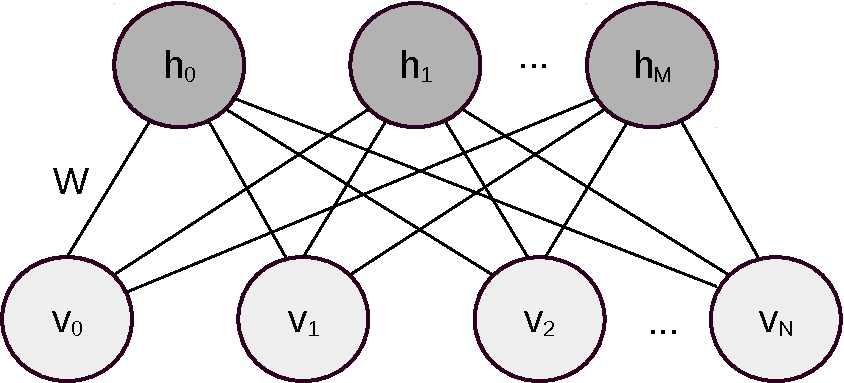
\includegraphics[width=0.6\textwidth]{pics_sdlm/rbm_o.pdf}
	\caption{A typical RBM structure.}
	\label{fig:RBM}
\end{figure}

Despite the various statistical models involved in RBMs and their training method, the actual training algorithm is rather simple thanks to the use of Contrastive Divergence~(CD)~\citep{hinton2002training}.
We can only illustrate some of the statistical models and sampling methods involved in RBM training, a detailed description can be found in~\citep{fischer2012introduction}. 
Stacked RBMs are also trained by layer-wise greedy algorithms, like stacked AEs, thus this section will focus on training a single RBM block.

\subsection{Energy-based Model}
In energy-based models, the probability of data point $x$ is defined by a model function $f(x)$, its energy function $E(x)$ and a partition function $Z$ which normalises the model function to possibilities by adding up all possible $f(x)$:
\begin{equation}
%\begin{aligned}
 p(x) = \dfrac{f(x)}{Z}~~, \textrm{~~where~~} f(x) =e^{-E(x)}~~,  \textrm{~~and~~}
 Z = \sum_{x} e^{-E(x)}~~.
%\end{aligned}
\end{equation} 
The energy function~\citep{hopfield1982neural} of a RBM is defined as follows:
\begin{equation}
E(\mathbf{v}, \mathbf{h} \mid \Theta)= -\sum_{i=1}^N a_i v_i - \sum_{j=1}^M b_j h_j - \sum_{i=1}^N \sum_{j=1}^M v_i w_{ij} h_j~~,
\label{equ:energy_complete}
\end{equation}
where the visible layer has $ N $ units, hidden layer has $ M $, and $ \Theta$ are the model parameters used in RBMs $ \Theta =\{\mathbf{a}, \mathbf{b}, \mathbf{w}\} $ including biases on visible layer, $\mathbf{a}$, hidden layer, $\mathbf{b}$, and weights between the layers $\mathbf{w}$.
As mentioned in Section~\ref{sec:spike}, for simplicity we use neurons without biases in this thesis.
Therefore only the third term of the complete energy function~(Equation~\ref{equ:energy_complete}) is kept:
\begin{equation}
E(\mathbf{v}, \mathbf{h} \mid \Theta)= - \sum_{i=1}^N \sum_{j=1}^M v_i w_{ij} h_j~~,
\label{equ:rbm_energy}
\end{equation}
and the model parameters are reduced to  $ \Theta = \{\mathbf{w}\} $.
Thus the joint probability of the visible vector (input) $\mathbf{v}$ and the output of hidden units $\mathbf{h}$ is defined as follows: 
\begin{equation}
\begin{aligned}
p(\mathbf{v}, \mathbf{h} \mid \Theta) &=\frac{f(\mathbf{v}, \mathbf{h} \mid \Theta)}{Z(\Theta)}~,  \textrm{~where~} \\
f(\mathbf{v}, \mathbf{h} \mid \Theta) &=e^{-E(\mathbf{v}, \mathbf{h} \mid \Theta)}~,  \textrm{~and~} \\
Z(\Theta) &= \sum_{\mathbf{v}} \sum_{\mathbf{h}} e^{-E(\mathbf{v}, \mathbf{h} \mid \Theta)}~.
\end{aligned}
\label{equ:rbm_prob}
\end{equation}
%However, we are more interested in the marginal probability function: $ p(\mathbf{v} \mid \Theta) $:
%\begin{equation}
%p(\mathbf{v} \mid \Theta) =\frac{\sum_{ \mathbf{h}} e^{-E(\mathbf{v}, \mathbf{h} \mid \Theta)}}{Z(\Theta)}~~,
%\end{equation}	

\subsection{Objective Function}
Given a set of outcomes data $ \mathbf{D}=\{\mathbf{v}^1, \mathbf{v}^2, ..., \mathbf{v}^K\} $, the likelihood function of model parameters $\Theta$ defines the probability of the outcomes $ \mathbf{D}$ given $\Theta$:
\begin{equation}
L (\Theta \mid \mathbf{D}) = p(\mathbf{D} \mid \Theta ) = \prod_{k=1}^K p(\mathbf{v}^k \mid \Theta ) =  \prod_{k=1}^K\dfrac{f(\mathbf{v}^k \mid \Theta )}{Z( \Theta)}~~.
\label{equ:likelihood}
\end{equation}
Thus the objective is to maximise the likelihood $L (\Theta \mid \mathbf{D})$ that is to say, the model parameters $ \Theta $ best defines the given data $\mathbf{D}$.
Furthermore, in order to simplify the product on the right-hand term in Equation~\ref{equ:likelihood} the objective function can be replaced with the average log-likelihood:
\begin{equation}
\label{equ:like}
\hat{l} (\Theta \mid \mathbf{D}) =\frac{1}{K}\log  L (\Theta \mid \mathbf{D}) 
=\frac{1}{K}\sum_{k=1}^K\log f(\mathbf{v}^k \mid \Theta ) - \log Z( \Theta)~~.
\end{equation}

%Note that, both visible and hidden units have their bias individually, $ \mathbf{a} $ and $ \mathbf{b} $.
%Thus the RBM consists of the data $ \mathbf{D} = \mathbf{V} = (\mathbf{v}_1, \mathbf{v}_2, ..., \mathbf{v}_K ) $, the model parameters $ \Theta = (\mathbf{a}, \mathbf{b}, \mathbf{w}) $ and the hidden units $ \mathbf{h} \sim p(\mathbf{h} \mid \mathbf{v}, \Theta) $.
%
%
%Here we take a Bernoulli-Bernoulli RBM as an example, where each node is a sigmoidal unit.
%The conditional probability function is as follows:
%\begin{equation}
%\begin{aligned}
%& p(h_j = 1 \mid \mathbf{v}) = \sigma(\sum_{i=1}^{M} w_{ij}  v_i + b_j)~,\\
%& p(v_i = 1 \mid \mathbf{h}) = \sigma(\sum_{j=1}^{N} w_{ji}  h_j + a_i)~.
%\end{aligned}
%\end{equation}


%SDG search in parameter space.
%
%Essentially, the integration of the probability model, see Equation~(\ref{equ:z_int}) and~(\ref{equ:z_dis}), is usually algebraically intractable.
%We have to use numerical integration method to evaluate the Equation~(\ref{equ:like}), whose partial derivative is (we are using vectors to generalise the problem):

The loss derivative with respect to a parameter $\theta$ is as follows:
\begin{equation}
\label{equ:part}
\begin{aligned}
\dfrac{\partial \hat{l} (\Theta \mid \mathbf{D})}{\partial \theta} 
& = \frac{1}{K} \dfrac{\partial \sum_{k=1}^K\log f(\mathbf{v}^k \mid \Theta )}{\partial \theta} - \dfrac{\partial \log Z( \Theta)}{\partial \theta}\\
& =  \frac{1}{K}\sum_{k=1}^K \dfrac{\partial \log f(\mathbf{v}^k \mid \Theta)}{\partial \theta} - \sum_x p(\mathbf{x} \mid \Theta) \dfrac{\partial \log f(\mathbf{x} \mid \Theta)}{\partial \theta}\\
& = \left \langle \dfrac{\partial \log f(\mathbf{v} \mid \Theta)}{\partial \theta}\right \rangle_{\mathbf{D}} -\left \langle \dfrac{\partial \log f(\mathbf{v} \mid \Theta)}{\partial \theta}\right \rangle_{\mathbf{C} \sim p(\mathbf{v} \mid \Theta)} ~~,
\end{aligned}
\end{equation}
where  $ <\cdot>_{\mathbf{X}} $ denotes the mean expectation of $ \cdot $ given data set $\mathbf{X}$.
The first term of the right-hand side is easy to get with the given data, $\mathbf{d} \in \mathbf{D} $, and the second term can be approximated by generating data samples $\mathbf{C} $ according to $ p(\mathbf{x} \mid \Theta) $.
%These generative samples is called ``fantasy data'' and can be generated using Monte Carlo Markov Chain (MCMC) sampling, see section~\ref{sec:mcmc}.
The detailed derivation process can be found in Appendix~\ref{app:part}.
%Although in this example the integration of product of normal distribution is still tractable, it is also helpful to use numerical integration.
%Although $ p(\mathbf{v} \mid \Theta) $ is not a PoE problem, the partial derivation of the average log-likelihood function still applies to Equation~(\ref{equ:part}) and the intractable integration is the same problem here:
Applying the model function of RBMs in Equation~\ref{equ:rbm_prob} to the loss derivative (Equation~\ref{equ:part}), Appendix~\ref{app:RBM} derives the loss function of RBMs in detail:
\begin{equation}
\label{equ:RBM}
\begin{aligned}
\dfrac{\partial \hat{l} (\Theta \mid \mathbf{D})}{\partial \theta} 
& = \left \langle \dfrac{\partial -E(\mathbf{v}, \mathbf{h} \mid \Theta)}{\partial \theta} \right \rangle_{\{\mathbf{D}, \mathbf{D}_h\} \sim p( \mathbf{h} \mid \mathbf{v}, \Theta)} 
- \left \langle \dfrac{\partial -E(\mathbf{v}, \mathbf{h} \mid \Theta)}{\partial \theta} \right \rangle_{\{\mathbf{C_v}, \mathbf{C_h}\} \sim p( \mathbf{v}, \mathbf{h} \mid  \Theta)},  \\
\end{aligned}
\end{equation}
Then we plug the energy function of RBMs (Equation~\ref{equ:rbm_energy}) into the equation above, the loss derivative with respect to the weight is:
\begin{equation}
\label{equ:RBM_2}
%\begin{aligned}
\dfrac{\partial \hat{l} (\Theta \mid \mathbf{D})}{\partial w_{ij}} 
= \left \langle v_i h_j \right \rangle_{\{\mathbf{D}, \mathbf{D}_h\} \sim p( \mathbf{h} \mid \mathbf{v}, \Theta)}
- \left \langle  v_i h_j \right \rangle_{\{\mathbf{C_v}, \mathbf{C_h}\} \sim p( \mathbf{v}, \mathbf{h} \mid  \Theta)}~~. %  \\
%\dfrac{\partial \hat{l} (\Theta \mid \mathbf{D})}{\partial a_{i}} 
%& = \left \langle v_i \right \rangle_{\mathbf{h} \sim p( \mathbf{h} \mid \mathbf{v}, \Theta), \mathbf{V}} 
%- \left \langle  v_i \right \rangle_{\mathbf{v}, \mathbf{h} \sim p( \mathbf{v}, \mathbf{h} \mid  \Theta)},  \\
%\dfrac{\partial \hat{l} (\Theta \mid \mathbf{D})}{\partial b_{j}} 
%& = \left \langle h_j \right \rangle_{\mathbf{h} \sim p( \mathbf{h} \mid \mathbf{v}, \Theta), \mathbf{V}} 
%- \left \langle  h_j \right \rangle_{\mathbf{v}, \mathbf{h} \sim p( \mathbf{v}, \mathbf{h} \mid  \Theta)},  \\
%\end{aligned}
\end{equation}
%\paragraph{CD with 1-step Reconstruction} 
\subsection{Weight update with Contrastive Divergence}
\label{sec:cd}
Generating data samples for the negative term of Equation~\ref{equ:RBM_2} requires Gibbs sampling on a Markov chain with infinite steps to convergence.
Gibbs sampling approximates the joint probability $p( \mathbf{v}, \mathbf{h} \mid  \Theta)$ with conditionally probability defined in RBMs:
\begin{equation}
\begin{aligned}
& p(h_j = 1 \mid \mathbf{v}) = \sigma(\sum_{i=1}^{M} w_{ij} v_i)~~,
& p(v_i = 1 \mid \mathbf{h}) = \sigma(\sum_{j=1}^{N} w_{ji} h_j)~~,
\end{aligned}
\label{equ:con_prob}
\end{equation} 
where $\sigma$ represents Sigmoid activation function for Bernoulli-Bernoulli RBMs.
Figure~\ref{fig:gibbs} illustrates the Gibbs sampling on an RBM by $k$ steps where each pair of $(\mathbf{v}, \mathbf{h})$ composes a state of the Markov chain, and the joint probability $p( \mathbf{v}, \mathbf{h} \mid  \Theta)$ is approximated by conditional probabilities embedded in the weights (Equation~\ref{equ:con_prob}).

\begin{figure}[hbt]
	\centering
	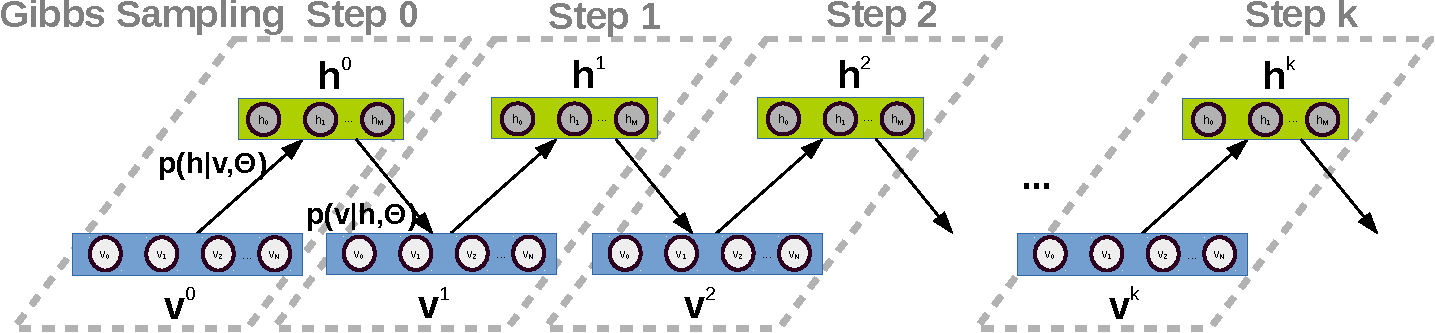
\includegraphics[width=0.98\textwidth]{pics_sdlm/gibbs_sampling.pdf}
	\caption{Gibbs sampling on a RBM.}
	\label{fig:gibbs}
\end{figure}

If $ k \to \infty $, the Markov chain will converge to an equilibrium which represents the distribution of the model-generated data $\{\mathbf{C_v}, \mathbf{C_h}\}$ described by the RBM, and Equation~\ref{equ:RBM} will represent the derivative of Kullback-Leibler~(KL) divergence with respect to parameter $\theta$.
The KL divergence measures the distance between two probability distributions: the training dataset $\{\mathbf{D}, \mathbf{D_h}\}$ and the generated Gibbs samples, $\{\mathbf{C_v}, \mathbf{C_h}\}$.
However, if we just take a few steps, the KL divergence can be seen as a k-step contrastive convergence ($ CD_{k}) $.
Even $ CD_1 $ has performed surprisingly well in RBM training~\citep{hinton2002training}.
Hence the RBM training using SGD is as follows :
\begin{equation}
\Delta w_{ij} = \eta (v^0_i h^0_j-v^1_i h^1_j)~~.
\label{equ:rbm_train}
\end{equation}



%The second term is perfect fit for Gibbs sampling, since we can $ p(\mathbf{v}, \mathbf{h} \mid \Theta) $ as a 2D vector and generating the samples by jumping in a Markov Chain with the transformation probability matrix $ p(\mathbf{v} \mid \mathbf{h}, \Theta) $ and $ p(\mathbf{h} \mid \mathbf{v}, \Theta) $, see Figure~\ref{fig:gibbs} and Section~\ref{sec:Gibbs}.
%So, with the given data $ \mathbf{v}_0 $ and the sampling data $ \mathbf{h}_0 $, we have the initial data point in this Markov Chain,  ($ \mathbf{v}_0, \mathbf{h}_0$).
%The transformation starts from the axis of $ \mathbf{v} $, then we get $ \mathbf{v}_1 \sim p( \mathbf{v} \mid \mathbf{h}_0, \Theta) $.
%It follows the next axis $ \mathbf{h} $, similarly we get $ \mathbf{h}_1 \sim p( \mathbf{h} \mid \mathbf{v}_1, \Theta) $.
%So far we obtain the first sample along the Markov Chain, ($ \mathbf{v}_1, \mathbf{h}_1$) thus to solve the objective function with one iteration.
%The algorithm is described below:   
%\begin{algorithm}[h]
%	\caption{Learning on RBM Parameters with $ CD_1 $}
%	\label{alg:learn}
%	\begin{algorithmic}
%		%			\State Initialisation $\mathbf{x}_0 = [x_0(1),x_0(2),...,x_0(M)]$,  \Comment{Random initialise $\mathbf{x}_0$}
%		\For{$t=1, 2, ..., K$} \Comment{K number of training data $ \mathbf{V} $, 1 data each iteration}
%		%			\For{$k=1, 2, ..., M$}
%		\State $ \mathbf{h}_t \sim p( \mathbf{h} \mid \mathbf{v}_t, \Theta) $
%		\Comment{Generate $ \mathbf{h}_t $ given $ \mathbf{v}_t $ }
%		\State $ \mathbf{v}_{t+1} \sim p( \mathbf{v} \mid \mathbf{h}_{t}, \Theta) $
%		\Comment{Generate $ \mathbf{v}_{t+1} $ on v axis using Gibbs sampling }
%		\State $ \mathbf{h}_{t+1} \sim p( \mathbf{h} \mid \mathbf{v}_{t+1}, \Theta) $
%		\Comment{Generate $ \mathbf{h}_{t+1} $ on h axis using Gibbs sampling }
%		\State $ \dfrac{\partial \hat{l} (\Theta \mid \mathbf{D})}{\partial W_{ij}} = v_{t,i} h_{t,j} - v_{t+1,i} h_{t+1,j}$
%		\State $ \dfrac{\partial \hat{l} (\Theta \mid \mathbf{D})}{\partial a_{i}} = v_{t,i} - v_{t+1,i} $
%		\State $  \dfrac{\partial \hat{l} (\Theta \mid \mathbf{D})}{\partial b_{j}} = h_{t,j} - h_{t+1,j}$
%		\State $ \Delta W_{ij} = \eta ( v_{t,i} h_{t,j} - v_{t+1,i} h_{t+1,j}) $
%		\Comment{Update $ W_{ij} $}
%		\State $ \Delta a_{i} = \eta ( v_{t,i} - v_{t+1,i}) $
%		\Comment{Update $ a_{i} $}
%		\State $ \Delta b_{j} = \eta ( h_{t,j} - h_{t+1,j}) $
%		\Comment{Update $ b_{j} $}
%		%			\EndFor
%		\EndFor
%	\end{algorithmic}
%	\label{alg:rbm}
%\end{algorithm}

\section{Summary}
This chapter briefly introduced the most popular deep learning techniques and models for potential use in spiking neural networks.
We illustrated the structure and training procedure for three deep learning models: Convolutional networks, Autoencoders and Restricted Boltzmann Machines, which will be applied in spiking deep networks in the following chapters.